\documentclass[10pt]{article}
\usepackage{titlesec}
\usepackage{geometry}
\geometry{verbose,tmargin=.9in,bmargin=.9in,lmargin=1.0in,rmargin=1.0in}
\usepackage{amsmath,amsfonts,amsthm,amssymb}
\usepackage{url}
\usepackage{color}
\usepackage[usenames,dvipsnames,svgnames,table]{xcolor}
\usepackage[colorlinks=true, linkcolor=red, urlcolor=blue, citecolor=gray]{hyperref}
\usepackage{float}
\usepackage{caption}
\usepackage{subcaption}
\usepackage{graphicx}
\usepackage{wrapfig}
\usepackage{booktabs}
\usepackage{longtable}
\usepackage{enumitem}
\usepackage{multicol}
\usepackage{etoolbox}
\usepackage{soul}
\captionsetup[subfigure]{labelformat=empty}
\captionsetup[figure]{labelformat=empty}

\definecolor{nyuDarkPurple}{HTML}{330662}
\definecolor{nyuOfficialPurple}{HTML}{57068c}

\newcommand{\spara}[1]{\vspace{.5em}\noindent {\large\sffamily\textcolor{nyuOfficialPurple}{#1}}}
\titleformat{\section}[hang]{\Large\sffamily\color{nyuDarkPurple}}{\thesection}{1em}{}
\titleformat{\subsection}[hang]{\large\sffamily\color{nyuDarkPurple}}{\thesection}{1em}{}
\titleformat{\subsubsection}[hang]{\normalsize\sffamily\color{gray}}{\thesection}{1em}{}

\usepackage{fancyhdr}
\pagestyle{fancy}
\lhead{
\includegraphics[width=4cm]{tandon_long_color.eps}}
\rhead{\thepage}
\pagenumbering{gobble}
\newcommand{\bs}[1]{\boldsymbol{#1}}
\newcommand{\bv}[1]{\mathbf{#1}}
\DeclareMathOperator*{\argmin}{arg\,min}
\DeclareMathOperator*{\argmax}{arg\,max}
\DeclareMathOperator*{\cut}{cut}
\DeclareMathOperator*{\sign}{sign}
\DeclareMathOperator*{\Var}{Var}
\DeclareMathOperator*{\tr}{tr}

\setcounter{secnumdepth}{0}

% math commands
\DeclareMathOperator{\R}{\mathbb{R}}
\newcommand{\E}{\mathbb{E}}

\begin{document}
	
\begin{center}
	\normalsize
	New York University Tandon School of Engineering
	
	Computer Science and Engineering
	\medskip
	
	\large
	CS-GY 6763: Final Exam. 
	
	Friday, Dec. 22nd, 2023, 2:00 - 3:30pm 
	
	(90 minutes, 18 minutes per question)
	\medskip
\end{center} 

\vspace{-3em}
\subsection{Directions}
\begin{itemize}
	\item Show all of your work to receive full (and partial) credit.
	\item If more space is required, you may use extra sheets of paper, clearly marked with your name and the problem you are working on.
	\item There are 5 multipart questions worth \textbf{60 points total}. 
\end{itemize}

\subsection{1. Always, Sometimes, Never}
\textbf{(15 pts, 3 per question)} Indicate whether each of the following statements is ALWAYS true, SOMETIMES true, or NEVER true. \textbf{Provide a short justification or example to explain your choice.} 
\begin{enumerate}[label=(\alph*)]		
		\item Given a matrix $\bv{V} \in \R^{n\times k}$ with orthonormal columns, for all $\bv{x} \in \R^n$, $\|\bv{VV}^T\bv{x}\|_2 = \|\bv{x}\|_2$.
		
		ALWAYS\hspace{1em} SOMETIMES\hspace{1em} NEVER\vspace{5em}
		
		\item The center-of-gravity method optimizes convex functions with fewer gradient oracle calls then gradient descent. 
		
		ALWAYS\hspace{1em} SOMETIMES\hspace{1em} NEVER\vspace{5em}
		
		\item If $\bv{A}$ has rank $1$ then $\|\bv{A}\|_2 = \|\bv{A}\|_F$.  
		
		ALWAYS\hspace{1em} SOMETIMES\hspace{1em} NEVER\vspace{5em}
		
		\item Given two matrices $\bv{A}$ and $\bv{B}$ with top eigenvectors $\bv{a}_1$ and $\bv{b}_1$, if $\|\bv{A} - \bv{B}\|_2 \leq \epsilon$ then $\sin(\theta(\bv{a}_1,\bv{b}_1)) \leq \epsilon$.\footnote{Recall that $\theta(\bv{a}_1,\bv{b}_1)$ denotes the angle between the unit vectors $\bv{a}_1$ and $\bv{b}_1$.}
	
		
		ALWAYS\hspace{1em} SOMETIMES\hspace{1em} NEVER\vspace{5em}
	
		\item Let $f_1(x), \ldots, f_n(x)$ be $\beta$-smooth convex functions and let $g(x) = \frac{1}{n}\sum_{i=1}^n f_i(x)$ be their average. $g$ is $\beta$-smooth.
		
		ALWAYS\hspace{1em} SOMETIMES\hspace{1em} NEVER\vspace{5em}
\end{enumerate}

% \subsection{2. Combinining convex functions}
% \textbf{(9 pts)}Either prove or provide a counter-example that disproves the following statements:
% \begin{enumerate}[label=(\alph*)]		
% 	\item (3pts) For convex functions $f(x)$ and $g(x)$, $f(x) + g(x)$ is convex.\vspace{6em}
	
% 	\item (3pts) For convex functions $f(x)$ and $g(x)$, $f(x)\cdot g(x)$ is convex.\vspace{6em}
	
% 	\item (3pts) For convex functions $f(x)$ and $g(x)$, $f(g(x))$ is convex.\vspace{6em}
% \end{enumerate}



\subsection{2. Matrix Representations of Graphs and PSDness}

\textbf{(13 pts)} Suppose we have an undirected graph $G$ with $n$ nodes. Let $D$ denote the graph's diagonal degree matrix, let $A$ denote its adjacency matrix, and let $L = D-A$ denote its Laplacian.
\begin{enumerate}[label=(\alph*)]		
	\item (4pts) In class we proved that $L$ is always positive semidefinite. Prove that the \emph{normalized} Laplacian matrix, $D^{-1/2} L D^{-1/2}$ is also positive semidefinite for any $G$.\vspace{20em}
	
	\item (4pts) Consider the graph $G'$ obtained by adding one new edge to $G$. Let $L'$ be the Laplacian of the new graph. Prove that $L \preceq L'$.\vspace{20em}
	
	\item (5pts) Prove that, when when $G$ has at least one edge and \underline{no self loops}, $A$ is \emph{never} positive semidefinite.


\end{enumerate}

\newpage
\subsection{3. $\ell_{\infty}$ Constrained Optimization Oracles}
\textbf{(12 pts)} Consider the set $\mathcal{A} = \{\bv{x} \in \R^d: \|\bv{x}\|_{\infty} \leq 1\}$, where $\|\bv{x}\|_{\infty} = \max_{i\in 1,\ldots d} |x_i|$.
\begin{enumerate}[label=(\alph*)]		
	\item (3pts) Prove that $\mathcal{A}$ is convex. \vspace{16em}
	
	\item (3pts) Write an equation or pseudocode to implement a projection oracle for $\mathcal{A}$.  For any $\bv{x} \in \R^d$ your oracle should return the projection of $\bv{x}$ onto $\mathcal{A}$. \vspace{10em}


	\item (4pts) Write an equation or pseudocode to implement a separation oracle for $\mathcal{A}$. For any $\bv{x}\notin \mathcal{A}$, prove that your oracle returns a valid separating hyperplane.
	 \vspace{22em}
	 
	 
	 \item (2pts) Suppose $f$ is a convex function and we want to minimize $f(x)$ subject to $x\in \mathcal{A}$. What is \textbf{one example} of an algorithm that requires a projection oracle to solve the minimization problem? What is \textbf{one example}  of an algorithm that requires a separation oracle?
	 \vspace{16em}
\end{enumerate}

\newpage
\subsection{4. Matrix Spectra}
	\textbf{(8 pts)} Suppose we have $100\times 100$  matrices $\bv{A}_1, \bv{A}_2,$ and $\bv{A}_3$ with singular value matrices $\bs{\Sigma}_{\bv{A}}$, $\bs{\Sigma}_{\bv{B}}$, and $\bs{\Sigma}_{\bv{C}}$, respectively. The diagonal values in these matrices are plotted and some specific numbers are shown below. 
		
		\noindent\begin{minipage}[c]{0.49\textwidth}
			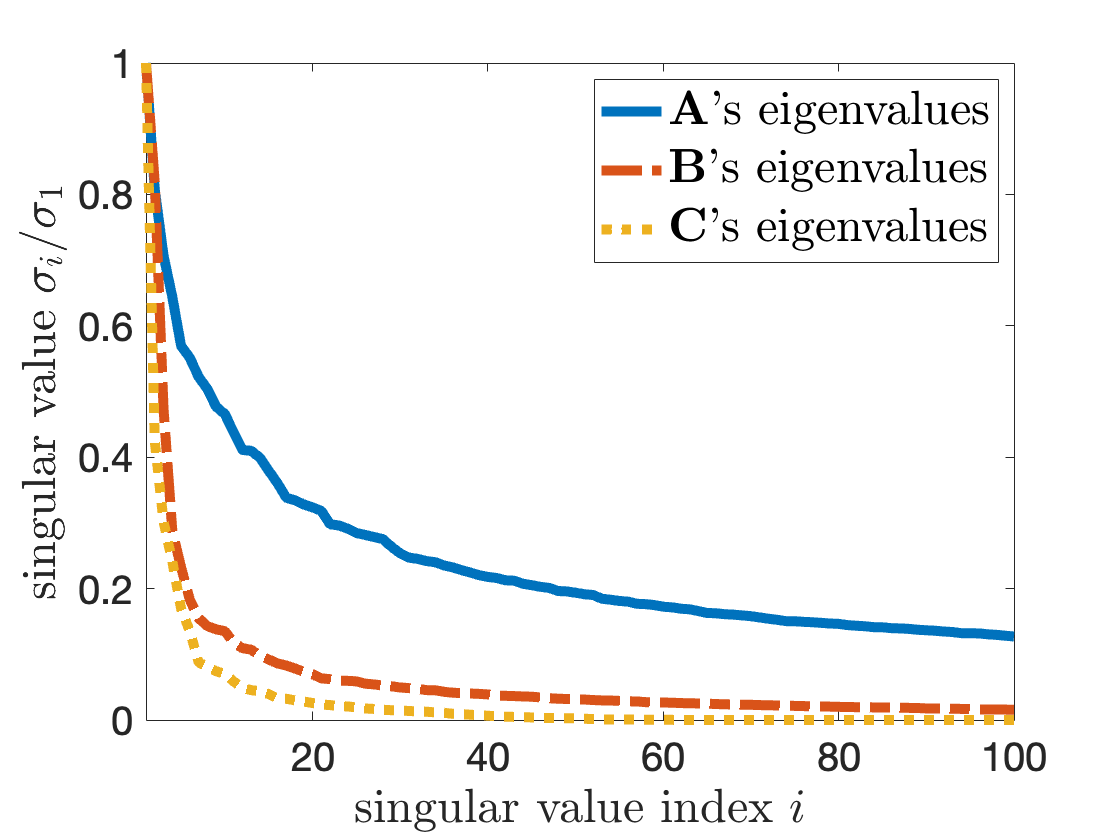
\includegraphics[width=.9\textwidth]{spectranew.png}
		\end{minipage}%
		\begin{minipage}[c]{0.49\textwidth}
			\Large
			\begin{align*}
				\bs{\Sigma}_{\bv{A}}&= [1,.81, .71, .64, \ldots, .21, .2]\\
				\bs{\Sigma}_{\bv{B}}&= [1,.82, .47, .29,  \ldots,.02,.01]\\
				\bs{\Sigma}_{\bv{C}} &= [1,.42, .30, .24, \ldots, .001, .001]\\
			\end{align*}
		\end{minipage}
		\vspace{2em}
\begin{enumerate}[label=(\alph*)]
		\item (2pts) Rank the matrices in order of which  would be best approximated by a rank-$40$ approximation. Justify your ranking.
	\vspace{11em}
	
		\item (3pts)  We want to find the top right singular vector of $\bv{A}, \bv{B},$ and $\bv{C}$ using the \textbf{power method}. Rank the matrices in order of which one you expect the method to converge faster for. Justify your ranking.
			\vspace{11em}
		
		\item (3pts)  We want to  solve the linear systems $\min_{\bv{x}} \|\bv{A}\bv{x} - \bv{y}\|_2, \min_{\bv{x}} \|\bv{B}\bv{x} - \bv{y}\|_2,$ and $\min_{\bv{x}} \|\bv{C}\bv{x} - \bv{y}\|_2$ using \textbf{gradient descent}.  Rank the matrices in order of which one you expect the method to converge faster for. Justify your ranking.
	\vspace{11em}		

		
\end{enumerate}

%\subsection{Problem 4: Faster Trace Estimation}
%\textbf{(15 pts)} As seen on Problem Set 3, a common task in linear algebra is to approximately compute the trace $\tr(\bv{A})$ of a matrix $\bv{A} \in \R^{n\times n}$ that you do not have explicit access to, but can multiply vectors by efficiently. We analyzed a randomized algorithm that constructed vectors $\bv{x}_1,\ldots, \bv{x}_m \in \R^n$ with uniformly random $\pm 1$. We proved that the estimator $\tilde{t} = \frac{1}{m}\sum_{i=1}^m \bv{x}_i^T(\bv{A}\bv{x}_i)$ satisfies:
%\begin{align*}
%	\E[\tilde{t}] &= \tr(\bv{A}) & \Var[\tilde{t}] &\leq \frac{2}{m}\|\bv{A}\|_F^2. 
%\end{align*}  
%We concluded via Chebyshev's Inequality that if $m = O(1/\epsilon^2)$, then with prob. $9/10$, $\left|\tr(\bv{A}) - \tilde{t}\right|\leq \epsilon\|\bv{A}\|_F$. 
%
%The estimator $\tilde{t}$ can be implemented using $O(1/\epsilon^2)$ matrix-vector products with $\bv{A}$. {In this problem, you will analyze a better method that requires $O(1/\epsilon)$ matrix-vector products with $\bv{A}$.}
%\begin{enumerate}[label=(\alph*)]		
%	\item (2 pts) Assume $\bv{A}$ is symmetric and positive semi-definite with eigenvalues $\lambda_1 \geq \ldots \geq \lambda_n \geq 0$. Show that the inequality $\left|\tr(\bv{A}) - \tilde{t}\right|\leq \epsilon\|\bv{A}\|_F$ implies that $\tilde{t}$ gives a relative error approximation. I.e. with probability $9/10$:
%	\vspace{-1em}
%	\begin{align*}
%		(1-\epsilon)\tr(\bv{A}) \leq \tilde{t} \leq (1+\epsilon)\tr(\bv{A}).
%	\end{align*}
%This is a warmup since we already proved it on the  problem set.  I am asking you to reprove the claim. 	\textbf{Hint:}  Use the fact that  $\|\bv{A}\|_F^2 = \sum_{i=1}^n \lambda_i^2$ and $\tr(\bv{A}) = \sum_{i=1}^n \lambda_i$.\vspace{18em}
%	
%	\hrulefill
%	
%For a fixed $k$, let $\bv{V}_k\in \R^{n\times k}$ contain the top eigenvectors of $\bv{A}$ (which are the same as it singular vectors since $\bv{A}$ is symmetric PSD). Observe that 
%\begin{align*}
%	\tr(\bv{A}) = \tr(\bv{A} - \bv{A}\bv{V}_k\bv{V}_k^T) + \tr(\bv{A}\bv{V}_k\bv{V}_k^T)
%\end{align*}
%
%We are going to design a faster trace estimation algorithm by estimating these two terms separately. In fact, we will focus only on the first term for this problem. We will assume that the second can be computed exactly using $O(k)$ matrix-vector products.\footnote{It is possible to rigorously address the case when $\bv{V}_k$ is only computed approximately, but I'm not asking you to do that here. For the sake of this problem, assume $\bv{V}_k$ is computed exactly.} This is because using e.g. Block Power Method, $\bv{V}_k$ can be approximated very accurately using $O(k)$ matrix-vector products. Once computed, we can then compute $\tr(\bv{A}\bv{V}_k\bv{V}_k^T)$ exactly using just $k$ matrix-vector products (to multiply $\bv{A}\bv{V}_k$).
%
%So, on the next page we turn our attention to approximating $\tr(\bv{A} - \bv{A}\bv{V}_k\bv{V}_k^T)$.
%\vspace{8em}
%
%		
%		
%		
%	\item  (6 pts) Prove that $\|\bv{A} - \bv{A}\bv{V}_k\bv{V}_k^T\|_F^2 \leq \epsilon \tr(\bv{A})^2$ for $k=1/\epsilon$. \textbf{Hint:} Write the left hand side as a sum involving eigenvalues. \vspace{22em}
%	
%	\item (3 pts) Argue that using $m = O(1/\epsilon)$ matrix vector multiplications with $\bv{A}$, it is possible to find some estimate $\tilde{z}$ such that with probability $9/10$:
%	\begin{align*}
%		\left|\tilde{z} - \tr(\bv{A} - \bv{A}\bv{V}_k\bv{V}_k^T) \right| \leq \epsilon \tr(\bv{A}).
%	\end{align*}
%\vspace{18em}
%	
%	\item (2pts) Use (b) and (e) to argue that that with $O(1/\epsilon)$ matrix-vector multiplications total we can find some $\tilde{t}$ such that with probability $9/10$, $(1-\epsilon)\tr(\bv{A}) \leq \tilde{t} \leq (1+\epsilon)\tr(\bv{A})$.
%\end{enumerate}

\newpage
\vspace{12em}
\subsection{Problem 5: Block Sparse Recovery}
\textbf{(12 pts)} In addition to being sparse, many vectors in practice (images, Fourier transforms, etc.) exhibit \emph{block structure}, where non-zeros are contained in contiguous blocks. We call a vector $\bv{x}\in \R^n$ \emph{$(k,q)$-block sparse} if 1) $\bv{x}$ has at most $kq$ non-zero entries and 2) all of those non-zeros are contained in \ul{at most} $q$ blocks of \ul{at most} $k$ consecutive indices. For example, the following two vectors are $(4,1)$-block sparse:
\begin{align*}
	\bv{x}_1 &= [0,0,\underbrace{1,-2,3,.5,}_{\text{block } 1}0,0,0] & \bv{x}_2 &= [\underbrace{.1,.3,-4,2,}_{\text{block } 1}0,0,0,0,0] 
\end{align*}
The following vectors are $(3,2)$-block sparse:
\begin{align*}
	\bv{x}_3 &= [\underbrace{3,-1,2,}_{\text{block } 1}0,\underbrace{.1,-9,1,}_{\text{block } 2}0,0] & \bv{x}_2 &= [0,\underbrace{-4,2,}_{\text{block } 1}0,0,0,\underbrace{.5,-6,7}_{\text{block } 2}] & \bv{x}_5 &= [0,\underbrace{1,-1,2}_{\text{block } 1},\underbrace{5,3,}_{\text{block } 2}0,0,0,0] 
\end{align*}

\begin{enumerate}[label=(\alph*)]		
	\item (2 pts) We say a matrix $\bv{A}\in \R^{m\times n}$ satisfies the $(k,q,\epsilon)$-block-RIP property if for \emph{all} $(k,q)$-block sparse vectors $\bv{x}$, \vspace{-1em}
	\begin{align*}
		(1-\epsilon)\|\bv{x}\|_2^2 \leq \|\bv{A}\bv{x}\|_2^2 \leq (1+\epsilon)\|\bv{x}\|_2^2.
	\end{align*} 
Since any $(k,q)$-block sparse vector is $kq$ sparse, a matrix $\bv{A}\in \R^{m\times n}$ satisfies the $(k,q,\epsilon)$-block-RIP property if it satisfies the $(kq,\epsilon)$-RIP property. If $\bv{A}$ is a random Johnson-Lindenstrauss  matrix, how many rows $m$ does it need to satisfy the $(kq,\epsilon)$-RIP property with probability 9/10? \textbf{Your answer should be in big-Oh notation.} \vspace{5em}
	
	\item (6 pts) Improve on your bound above by proving that, with probability $9/10$), a random Johnson-Lindenstrauss matrix with $O\left(\frac{kq + q\log(n/q)}{\epsilon^2}\right)$ rows satisfies the $(k,q,\epsilon)$-block-RIP property. \textbf{Hint:} Use the Subspace Embedding theorem.
%Note that all $(k,q)$-block sparse vectors are $kq$ sparse, so this improves on the general requirement of $O\left(\frac{kq\log n}{\epsilon^2}\right)$ rows for $(kq,\epsilon)$-RIP. 
	\vspace{21em}

	
	\item (4 pts)
Prove that if $\bv{A}$ satisfies the  $(k,2q,\epsilon)$-block RIP property for any $\epsilon <1$, then $\bv{x}$ is the \ul{unique} $(k,q)$-block sparse vector satisfying 	$\bv{b} = \bv{A}\bv{x}$. In other words, $\bv{x}$ can be recovered from the $m$ linear measurements in $\bv{b}$.
	\vspace{10em}
\end{enumerate}

% \newpage
% \vspace{12em}
% \subsection{Problem 5: Sketching Cuts}
% \textbf{(13 pts)}  Let $G$ be an unweighted undirected graph with vertex set $V$ and edge set $E$, where $|V| = n$. Let $\bv{B} \in \R^{|E|\times n}$ denote the graph's edge-vertex incidence matrix. Let $\bs{\Pi} \in \R^{m \times |E|}$ be a random Johnson-Lindenstrauss matrix with $m = O\left(\frac{\log(1/\delta)}{\epsilon^2}\right)$ rows (e.g. random Gaussian). Suppose we sketch $G$ by forming the $m \times n$ matrix $\bs{\Pi}\bv{B}$.

% \begin{enumerate}[label=(\alph*)]		
% 	\item (4 pts)
% 	Given any fixed vertex set $S \subseteq V$, describe and prove correct a method that can estimate $\cut(S,V\setminus S)$ up to $(1\pm \epsilon)$ multiplicative error with probability $1-\delta$ using the information in $\bs{\Pi}\bv{B}$. I.e., your method should return some estimate $\tilde{C}$ satisfying:
% 	\begin{align*}
% 		(1-\epsilon) \cdot\cut(S,V\setminus S) \leq \tilde{C} \leq 	(1+\epsilon) \cdot\cut(S,V\setminus S)
% 	\end{align*}
% \vspace{12em}

% 	\item (4 pts)
% Suppose we instead take $m = O\left(\frac{n + \log(1/\delta)}{\epsilon^2}\right)$. Show that, using the information in $\bs{\Pi}\bv{B}$, we can output a multiplicative approximation to $\cut(S,V\setminus S)$ for \emph{all sets $S$} simultaneously. 
% \vspace{13em}


% 	\item (3 pts) Argue that the sketch from (b) can be used to compute a multiplicative approximation to the minimum cut in $G$. I.e., describe how to compute some $\tilde{S}$ such that:
% 	\vspace{-.2em}
% 	\begin{align*}
% 		\cut(\tilde{S}, V\setminus \tilde{S}) \leq (1+O(\epsilon))\cdot \min_{S}\cut(\tilde{S}, V\setminus \tilde{S})
% 	\end{align*}
% 	\vspace{-2em}
	
% You algorithm does not need to be computationally efficient, but it must estimate the minimum cut using only the information in $\bs{\Pi}\bv{B}$.
% 	\vspace{11em}
	
% 	\item (2 pts) Would the guarantee of (a) suffice instead? I.e. could we approximate the minimum cut using a sketch with $mfin	in	i = O\left(\frac{\log(1/\delta)}{\epsilon^2}\right)$ rows?  Answer yes or no and explain your answer.

% \end{enumerate}

%\newpage
%\subsection{4. Sketching for Approximate Singular Vector Computation (\textbf{\small 10pts})}
%In this problem we are interested in approximating the \emph{last} singular vector of a matrix $\bv{A} \in \R^{n \times d}$ using a randomized sketching method. I.e. the vector corresponding to the smallest singular value. Specifically, we consider the setting when $n$ is much larger than $d$. 
%
%Let $\bs{\Pi} \in\R^{m \times n}$ be a random Johnson-Lindenstrauss matrix, e.g. with scaled random Gaussian or $\pm 1$ entries. Let $m = O\left(\frac{d + \log(1/\delta)}{\epsilon^2}\right)$. Let $\bv{v}_d$ be $\bv{A}$'s last right singular vector. Recall that $\bv{v}_d = \argmin_{\bv{v}: \|\bv{v}\|_2=1} \|\bv{A}\bv{v}\|_2$. We will approximate $\bv{v}_d$ by computing the last right singular vector of the smaller sketched matrix $\bs{\Pi}\bv{A}$.
%
%\begin{enumerate}[label=(\alph*)]
%%	\item (6pts) Let $\bv{\tilde v}_1$ be the first right singular vector of $\bs{\Pi}\bv{A}$. Prove that with probability $(1-\delta)$, $\|\bv{A}\bv{\tilde v}_1\|_2 \geq (1-\epsilon)\|\bv{A}\bv{v}_1\|_2$. In other words, $\bv{\tilde v}_1$ is a good approximate first singular vector.
%%	\vspace{14em}
%	%
%	\item (6pts) Let $\bv{\tilde v}_d$ be the last right singular vector of $\bs{\Pi}\bv{A}$.  that with probability $(1-\delta)$, $\|\bv{A}\bv{\tilde v}_d\|_2 \leq (1+\epsilon)\min_{\bv{v}: \|\bv{v}\|_2 = 1} \|\bv{A}\bv{v}\|_2$. In other words, $\bv{\tilde v}_d$ is a good approximate last singular vector.
%	\vspace{25em}
%	
%	
%	\item (4pts) What is the computational complexity of the approach described above for approximating the last singular vector of $\bv{A}\in \R^{n\times d}$. Is it faster than methods for computing an SVD of $\bv{A}$? What is one technique learned in class would make the sketching method faster?
%\end{enumerate}

%\newpage
%\subsection{5. Complete the Separation Oracle (\textbf{\small 12pts})}
%For a convex set $\mathcal{S}$ in $\R^d$, given any point $\bv{x}\notin \mathcal{S}$, a separation oracle must return a hyperplane $\mathcal{H}$ that separates $x$ from $\mathcal{S}$. Recall that a hyperplane has the equation $\mathcal{H} = \{\bv{y}: \bv{a}^T\bv{y} = c\}$, where $\bv{a}$ is a $d$ dimensional vector and $c$ is a scalar. 
% For both of the following questions, I describe a convex set $\mathcal{S}$, and tell you one possible choice of $\bv{a}$. Your job is to give a choice of $c$ so that the $\mathcal{H} = \{\bv{y}: \bv{a}^T\bv{y} = c\}$ is a hyperplane that separates $\bv{x}$ and $\mathcal{S}$. Note that $\bv{a}$ and $c$ will typically depend on $\bv{x}$. \textbf{Justify your answers for full credit. I.e., prove your chosen value of $c$ leads to a valid separating hyperlane.} 
%
%\begin{enumerate}[label=(\alph*)]
%	\item (6pts) Let $\mathcal{S} = \{\bv{z}: \|\bv{z}\|_1 \leq 1\}$. Let $\bv{x}$ be a point not in $\mathcal{S}$. There is a separating hyperplane for $\mathcal{S}, \bv{x}$ with parameters $\bv{a} = \sign(\bv{x})$ and $c=\ldots$
%	
%	\noindent \textbf{Note:} $\sign(\bv{x})$ denotes the vector which is $1$ in every entry where $\bv{x}$ is positive or zero and $-1$ in every entry where $\bv{x}$ is negative.
%	
%	\vspace{20em}
%	
%	\item (6pts) Let $\mathcal{S}$ be a convex set with projection oracle $\mathcal{P}$. I.e., for any $\bv{x}$, $\mathcal{P}(\bv{x})$ returns $\mathcal{P}(\bv{x})= \argmin_{\bv{z}\in \mathcal{S}} \|\bv{z} - \bv{x}\|_2$. Let $\bv{x}$ be a point not in $\mathcal{S}$. There is a separating hyperplane for $\mathcal{S}, \bv{x}$ with parameters $\bv{a} = \bv{x} - \mathcal{P}(\bv{x})$ and $c=\ldots$
%	
%	\noindent \textbf{Hint:} It might help to draw a picture. 
%
%\vspace{10em}
%\end{enumerate}





\end{document}